\documentclass[12pt]{article}
\usepackage{graphicx}
\usepackage{wrapfig}
\usepackage{hyperref}

\usepackage[style=phys,url=true]{biblatex}
\addbibresource{ref.bib}

\graphicspath{{Figures/}}
\addtolength{\textwidth}{1in}
\addtolength{\textheight}{1in}
\addtolength{\evensidemargin}{0.5in}
\addtolength{\oddsidemargin}{-0.5in}
\addtolength{\topmargin}{-0.5in}

\title{CTA200H Mini-Project: MW Analogues in Cosmological Simulations}
\author{Alicia Savelli\\Advisors: Ted Mackereth and Josh Speagle}
\date{\today}

\begin{document}
\maketitle

%\tableofcontents
%\clearpage 

\section{Introduction}
\begin{wrapfigure}{R}{0.7\textwidth}
    \centering
    \includegraphics[width=0.7\textwidth]{gms.png}
    \caption{Cartoon sketch of the GMS and outliers.  Majority of galaxies are pictured along the blue main sequence.  The outliers are grouped into high-rate star-forming galaxies (`starbursts') laying above the GMS in pink and low-rate star-forming galaxies (`red and dead') falling below the GMS in red~\cite{Alton2016}.}
    \label{fig:gms}
\end{wrapfigure}

The star-forming Galaxy Main Sequence (GMS) is a current and fairly recent topic of study in astronomy.  The GMS comes out of the relationship between galactic Stellar Mass (SM) and Star Formation Rate (SFR), as illustrated in Figure~\ref{fig:gms}.  In this model, the GMS is represented by the blue-shaded central grouping of galaxies along which majority of star-forming galaxies are thought to lie.  The remaining galaxies fall into the outlier groups `starburts', `the green valley', and `red and dead'.  The galaxies in the starbursts grouping have an exceptionally fast rate of star-formation; they are plotted in pink.  The low-rate star-forming galaxies are found in the green valley and the read and dead galaxies, pictured in green and red, respectively.  One current understanding of the GMS is that as the SM of a galaxy grows, so too does its SFR, until the dust needed for star-formation has been used up and the galaxy is said to be `quenched'.  At this stage, the galaxy `falls off' the main sequence and enters the green valley and the red and dead group, where star-formation is very low~\cite{Alton2016}.


The name `GMS' is reminiscent of the well-known stellar main sequence, although its relationship is not as well established.  The above interpretation is only one model of the GMS, and other studies have suggested both that the main sequence and the red and dead galaxies may be two separate groupings of galaxies, and that the groups may lie along a single smooth distribution~\cite{Eales_2016}.  Another factor to consider in the study of the GMS is the morphology of the galaxies along the distribution in relation to the Hubble sequence~\cite{Eales_2016}.   



The purpose of this mini-project was to become familiar with writing {\tt SQL} queries to pull data from the EAGLE galaxy formation simulations and analyze their output using {\tt matplotlib} in {\tt python}.  First, the SM and SFR of galaxies at redshift $z=0$ were plotted against each other in a variety of styles.  The graphs were analyzed and their features compared to physical observations of the GMS.  Then, SM and SFR of galaxies at redshift $0<z<0.5$ were plotted and analyzed.  This range in redshift corresponds to a lookback time of 5.19 billion years, and thus the data illustrates the formation and evolution of these galaxies through the merging of smaller galaxies at longer redshifts.   

\section{Methods and Results}
The study of the GMS was completed in two parts: analysis of data from the EAGLE simulations at $z=0$ and at $0\leq z <0.5$.  A description of the simulation and the data in the tables can be found in Reference~\cite{EAGLE}.  The script used to generate the figures and analyze the data can be found at \url{https://github.com/as14bq/CTA200/tree/master/project}.

\subsection{Retrieving EAGLE Galaxy properties: your first {\tt SQL} query in {\tt python}}

The initial query was coded as:
\begin{verbatim}
        SELECT sub.MassType_Star as stellar_mass, 
               sub.StarFormationRate as SFR,
               mag.r_nodust as r,
               mag.g_nodust as g
        FROM RefL0100N1504_SubHalo as sub,
             RefL0100N1504_Magnitudes as mag
        WHERE sub.SnapNum = 28 and
              sub.GalaxyID = mag.GalaxyID
\end{verbatim}
which imported the columns for SM, SFR, and the rest-frame absolute magnitudes in the \textit{g} and \textit{r} bands without dust attenuation from the {\tt RefL0100N1504\_SubHalo} and \\{\tt RefL0100N1504\_Magnitudes} tables for a {\tt Redshift} $z=0$, and joined the tables on {\tt GalaxyID}.  

\begin{figure}[htbp]
  \centerline{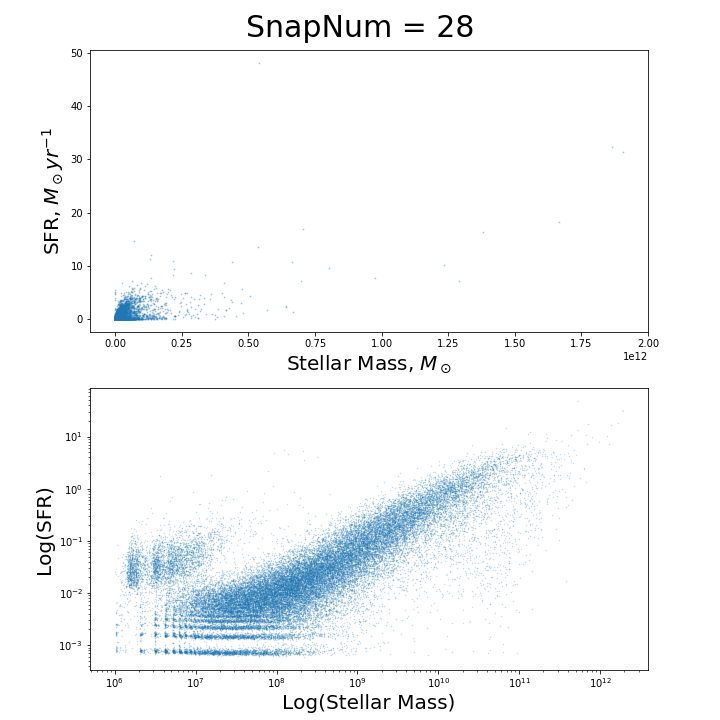
\includegraphics[width=0.6\textwidth]{SMvSFR.png}}
  \caption{Plot of the galactic Stellar Mass (SM) ($M_\odot$) against Star Formation Rate (SFR) ($M_\odot\rm{yr}^{-1}$) on linear scales (above) and logarithmic scales (below) at {\tt SnapNum = 28} ($z=0$).  A relationship between SM and SFR becomes visible in the loglog plot of the data.  The points have been made partially transparent so that the density of galaxies across the plot can be more easily observed.}
  \label{fig:SMvSFR}
\end{figure}

\begin{figure}[htbp]
  \centerline{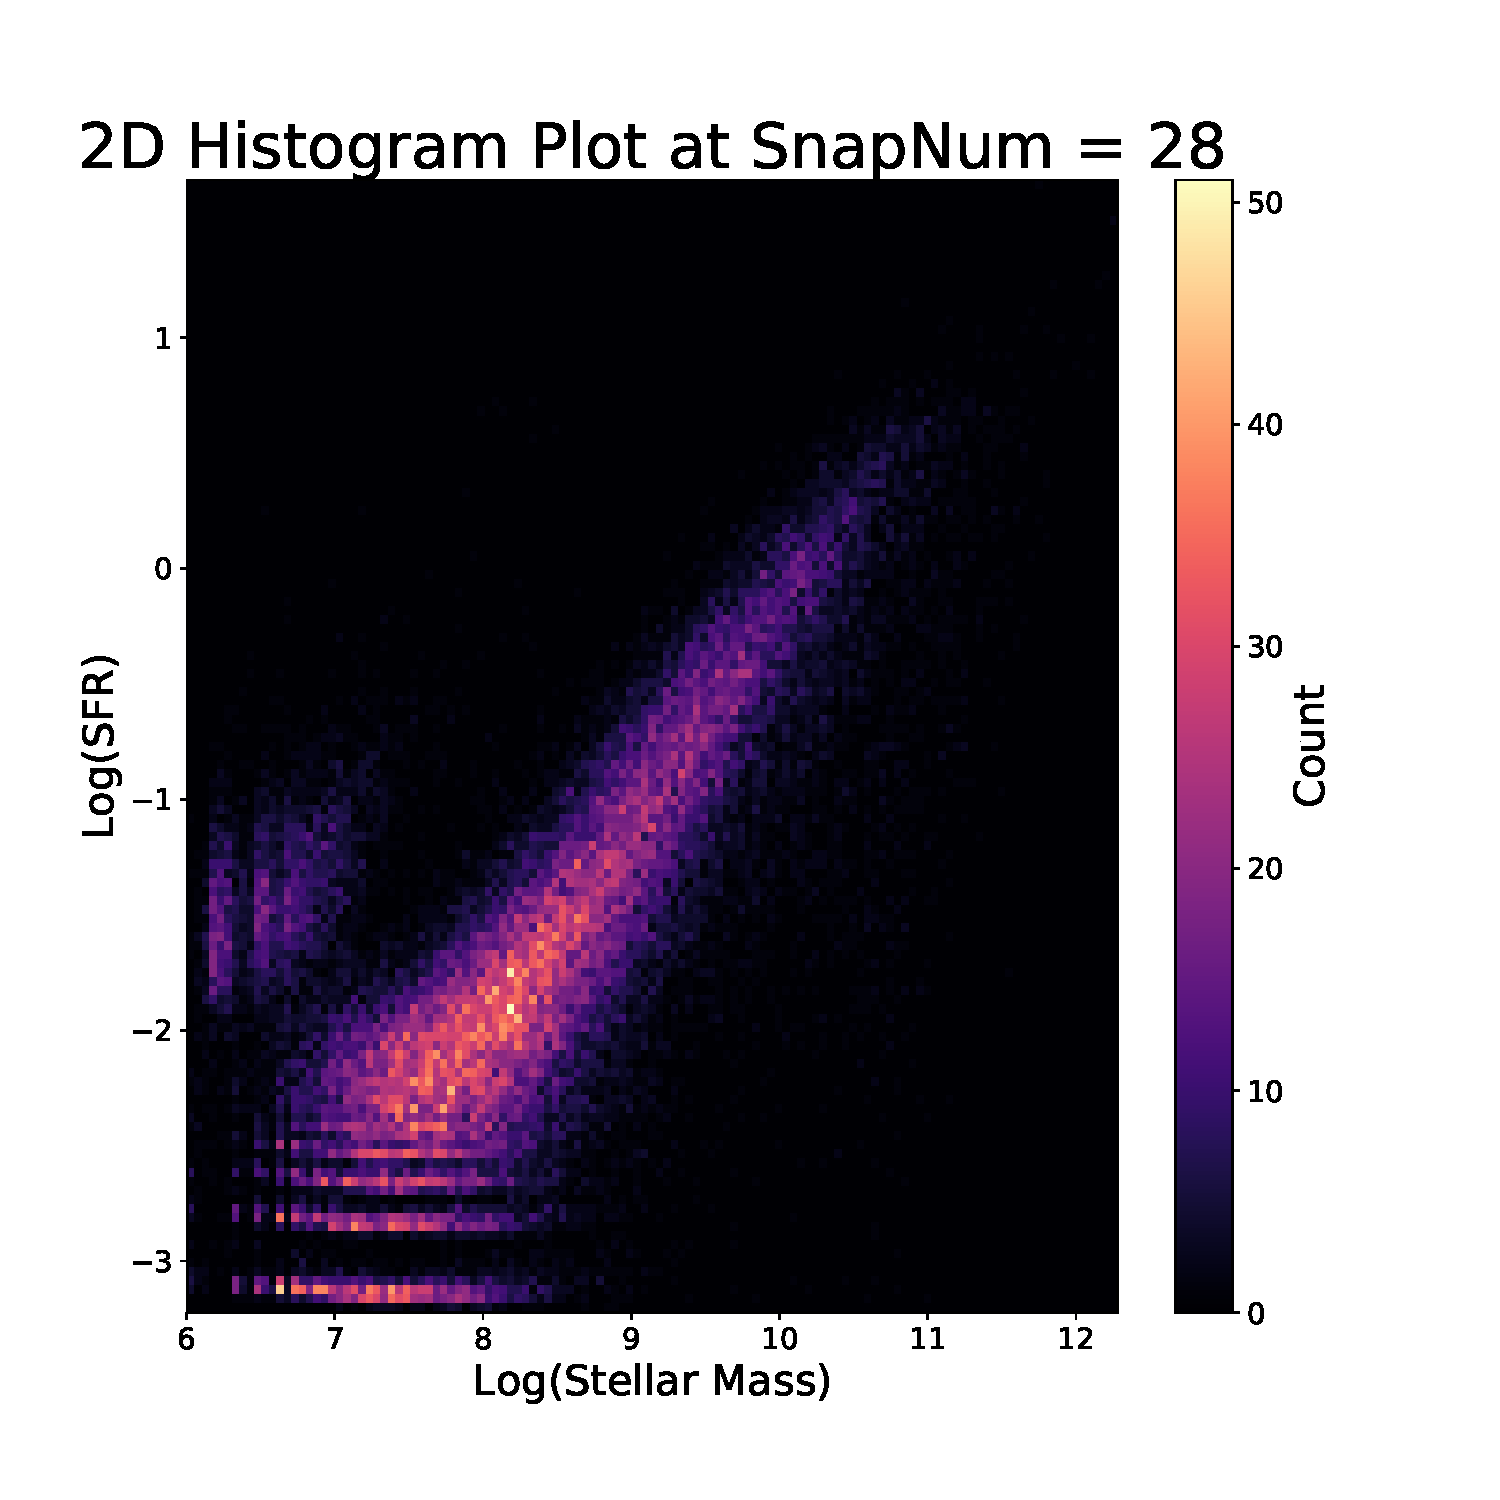
\includegraphics[width=0.5\textwidth]{hist.pdf}}
    \caption{Loglog histogram of the galactic Stellar Mass (SM) ($M_\odot$) against Star Formation Rate (SFR) ($M_\odot\rm{yr}^{-1}$) at {\tt SnapNum = 28} ($z=0$).  The figure shows a higher density of galaxies along the centre of the main sequence.}
    \label{fig:hist}
\end{figure}

\begin{figure}[htbp]
  \centerline{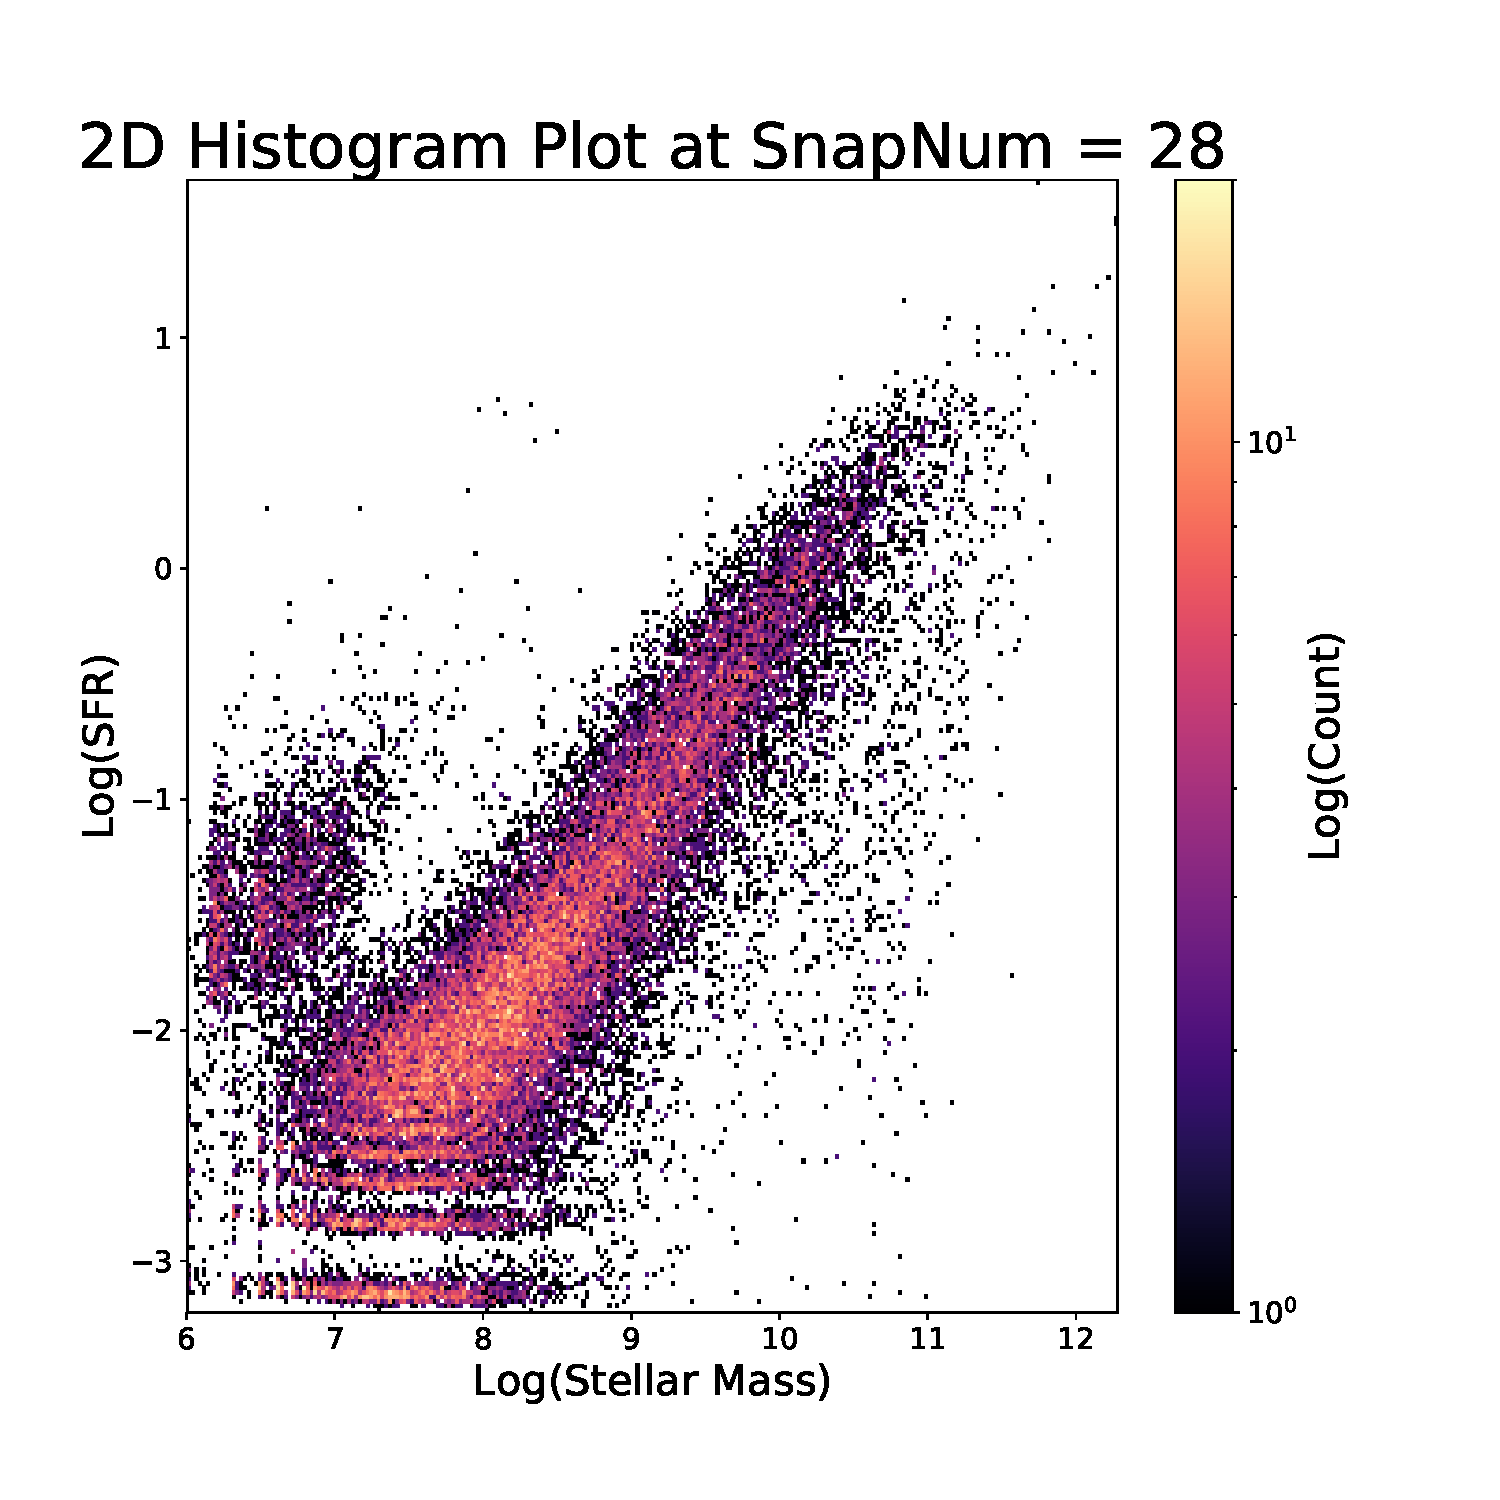
\includegraphics[width=0.5\textwidth]{histlog.pdf}}
    \caption{Loglog histogram of the galactic Stellar Mass (SM) ($M_\odot$) against Star Formation Rate (SFR) ($M_\odot\rm{yr}^{-1}$) with a logarithmic count at {\tt SnapNum = 28} ($z=0$).  The figure shows a higher density of galaxies along the centre of the main sequence.}
    \label{fig:histlog}
\end{figure}

\begin{figure}{0.5\textwidth}
    \centerling{includegraphics[width=0.5\textwidth]{colour.pdf}}
    \caption{Loglog plot of the galactic Stellar Mass (SM) ($M_\odot$) against Star Formation Rate (SFR) ($M_\odot\rm{yr}^{-1}$) coloured by $g-r$ colour at $z=0$.  The figure shows redder galaxies towards the bottom of the sequence and greener galaxies above.}
    \label{fig:colour}
\end{figure}


The script plotted the galactic Stellar Mass (SM) ($M_\odot$) against Star Formation Rate (SFR) ($M_\odot\rm{yr}^{-1}$) on both linear and logarithmic scales (Figure~\ref{fig:SMvSFR}).  The relationship between SM and SFR is not immediately obvious on the linear scaling, but with logarithmic axes there appears to be a sequence of galaxies where SFR increases with SM.  Although the opacity of the points was adjusted to give a better representation of the density, more representative loglog histograms of the data are presented in Figures~\ref{fig:hist} and~\ref{fig:histlog}, where the density is indicated by the colouring on a linear scale and a logarithmic scale, respectively.  These histogram plots give a better indication of the number of galaxies along the GMS.  A number of key features can be observed in all three of the loglog plots, as well as a few differences between them, all of which will be expanded upon in the Discussion section.    


A final analysis of the data taken at $z=0$ was a plot of the colour of the galaxies along the GMS.  The difference between the magnitudes of the galaxies in the green and red bands was taken to provide the colouring of the loglog plot in Figure~\ref{fig:colour}.


\subsection{Going Deeper into the Simulations: more properties and more snapshots}

The second part of the study examined galaxies at {\tt Redshift} $0 \leq z < 0.5$.  The query was coded as:
\begin{verbatim}
    SELECT MassType_Star as stellar_mass2, 
           StarFormationRate as SFR2,
           GalaxyID as galaxyID,
           TopLeafID as topleaf,
           LastProgID as lastprog,
           DescendantID as descID,
           Redshift as Z,
           Mass as mass
    FROM RefL0100N1504_SubHalo
    WHERE Redshift < 0.5
    ORDER BY GalaxyID
\end{verbatim}
where SM and SFR have again been pulled from table {\tt RefL0100N1504\_SubHalo}, along with the columns needed for analyzing the progenitors, the {\tt Redshift}, and the overall mass, for $0 \leq z < 0.5$, and the results were ordered by their {\tt GalaxyID}.

The same loglog plots from the first part of the study were run again for this higher volume of galaxies, with results illustrated in Figures~\ref{fig:SMvSFR2},~\ref{fig:hist2}, and~\ref{fig:histlog2}.  Similarities and differences between these same plots at $z=0$ and at $0 \leq z < 0.5$ will be explored in the Discussion section.  

\begin{figure}[htbp]
  \centerline{\includegraphics[width=0.8\textwidth]{tree.png}}
  \caption{Merger history of a galaxy with a $z = 0.18$ stellar mass M$_*$ $\sim 10^{10}$ M$_\odot$ indicated by the circled dot. Symbol colours and sizes are scaled with the logarithm of the stellar mass. The {\tt GalaxyID} of this galaxy points towards it, as indicated by the arrow. The main progenitor branch is indicated with a thick black line, all other branches with a thin line. The {\tt TopLeafID} gives the {\tt GalaxyID} of the highest redshift galaxy on the main progenitor branch whilst the {\tt LastProgID} (not shown) gives the maximum {\tt GalaxyID} of all the progenitors of the galaxy considered. Querying all galaxies with an ID between {\tt GalaxyID} and {\tt LastProgID} will return all the progenitor galaxies in the tree. (Taken verbatim from~\cite{EAGLE})}
  \label{fig:tree}
\end{figure}

With a larger range in redshift, the same galaxies can be analyzed across different times.  Figure~\ref{fig:tree}, taken from~\cite{EAGLE}, shows an example of a merger tree at $z=0.18$.  A merger tree shows all the past history of a given galaxy.  All of the past galaxies that have merged to give the present galaxy (progenitor galaxies) can be found from querying all galaxies with an ID between the given {\tt GalaxyID} and its {\tt LastProgID}.  The galaxy chosen to be analyzed was the most massive galaxy, of SM 1.9054253 $\times10^{12}$ M$_\odot$ and ID 21379521.  Analysis of the data found that there were 27 descendants of Galaxy 21379521 along the main branch, and 194064 total descendants.

\begin{figure}[htbp]
  \centerline{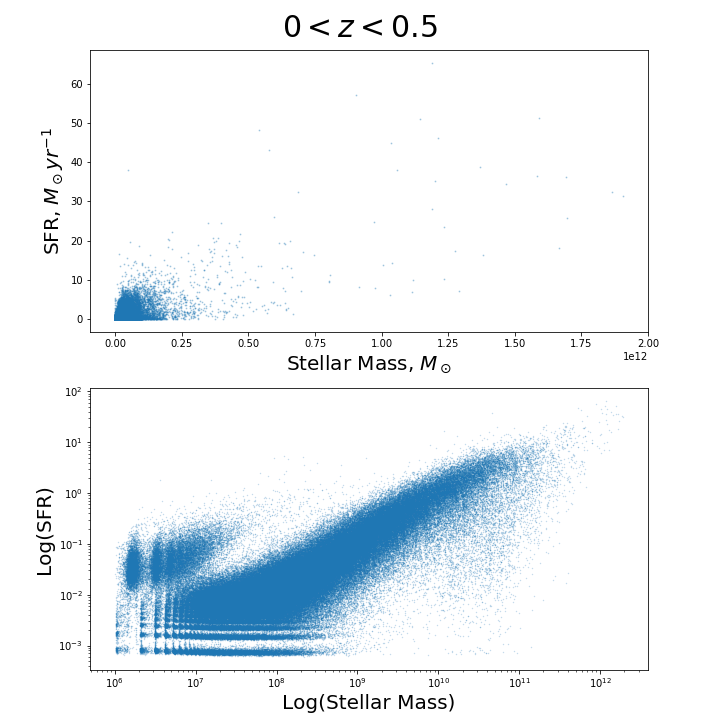
\includegraphics[width=0.6\textwidth]{SMvSFR2.png}}
  \caption{Plot of the galactic Stellar Mass (SM) ($M_\odot$) against Star Formation Rate (SFR) ($M_\odot\rm{yr}^{-1}$) on linear scales (above) and logarithmic scales (below) at $0\leq z < 0.5$.  A relationship between SM and SFR becomes visible in the loglog plot of the data.  The points have been made partially transparent so that the density of galaxies across the plot can be more easily observed.}
  \label{fig:SMvSFR2}
\end{figure}

\begin{figure}[htbp]
  \centerline{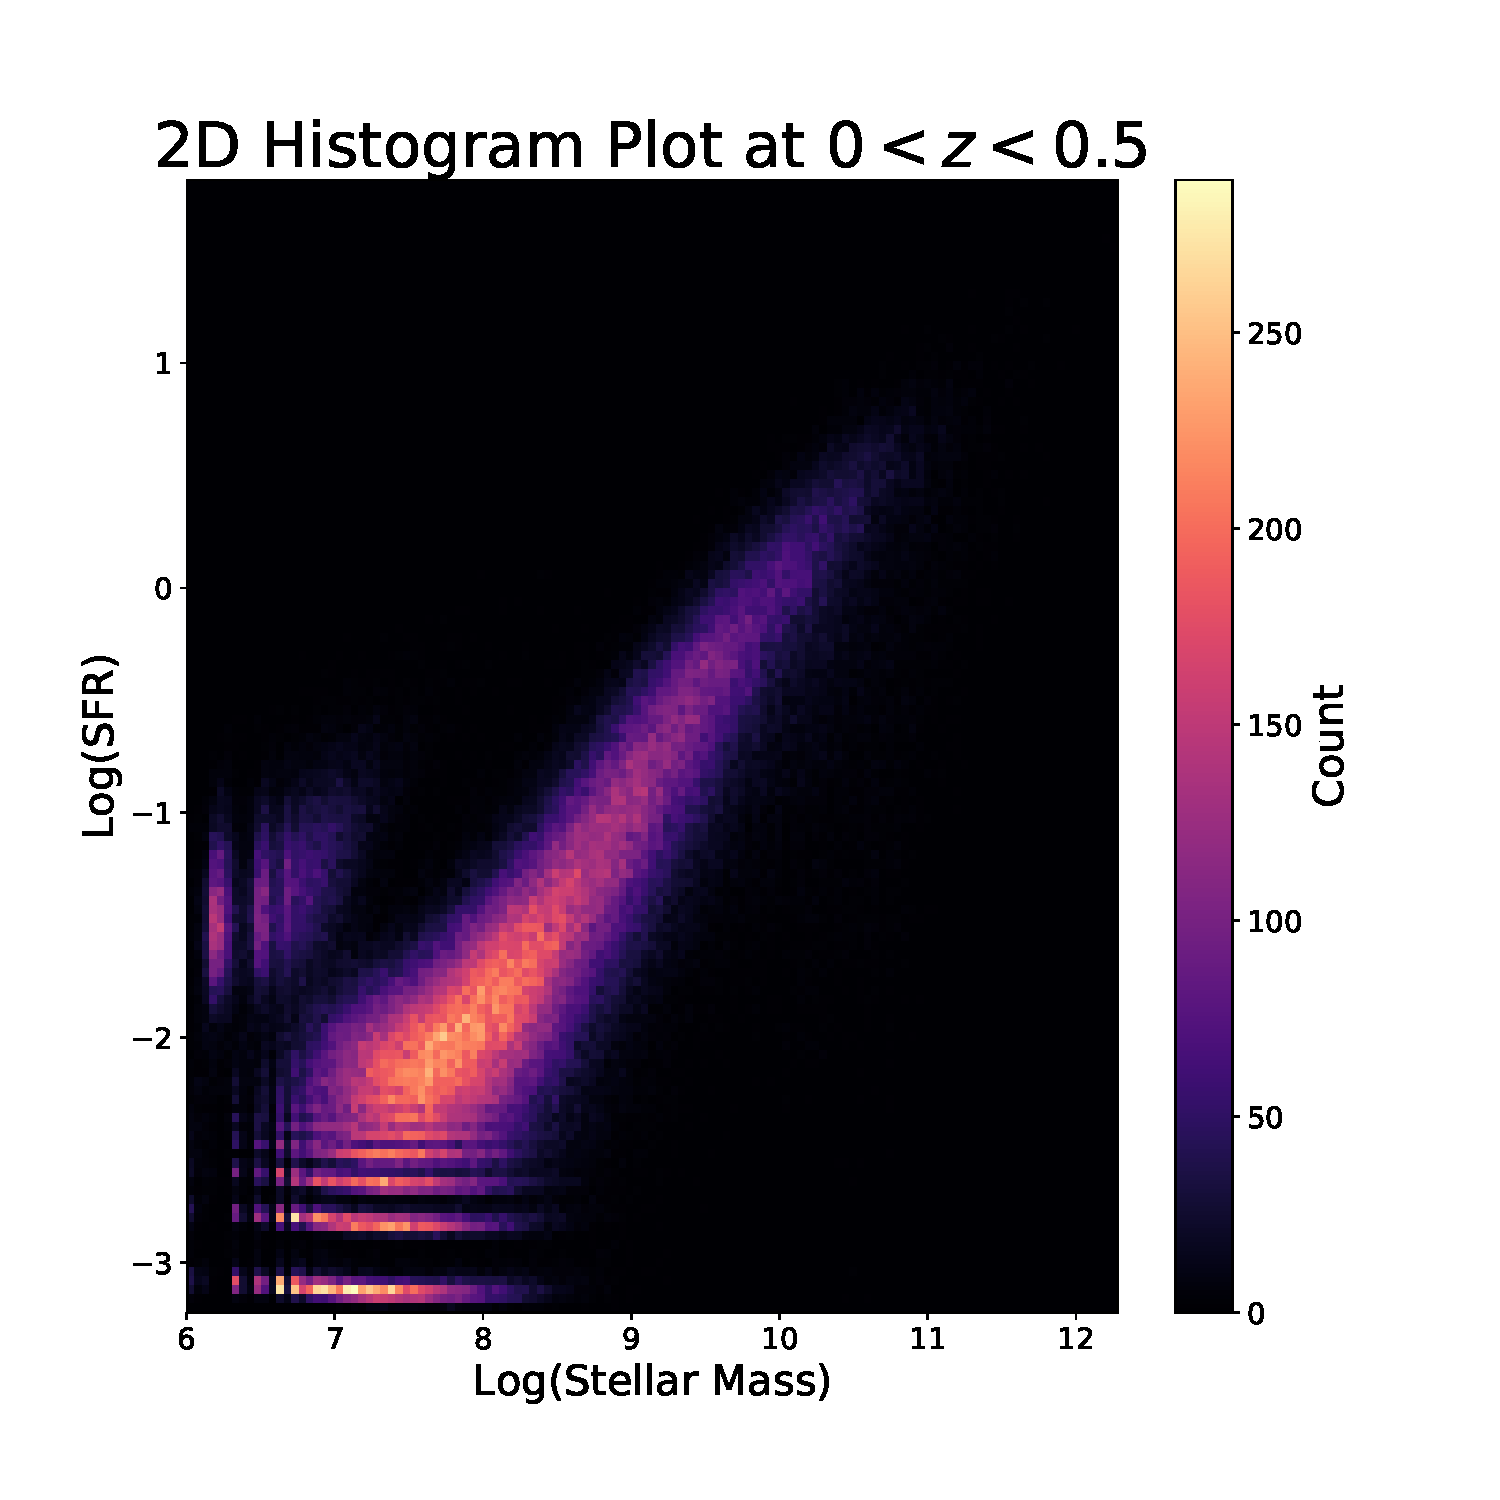
\includegraphics[width=0.5\textwidth]{hist2.pdf}}
    \caption{Loglog histogram of the galactic Stellar Mass (SM) ($M_\odot$) against Star Formation Rate (SFR) ($M_\odot\rm{yr}^{-1}$) at $0\leq z < 0.5$.  The figure shows a higher density of galaxies along the centre of the main sequence.}
    \label{fig:hist2}
\end{figure}

\begin{figure}[htbp]
  \centerline{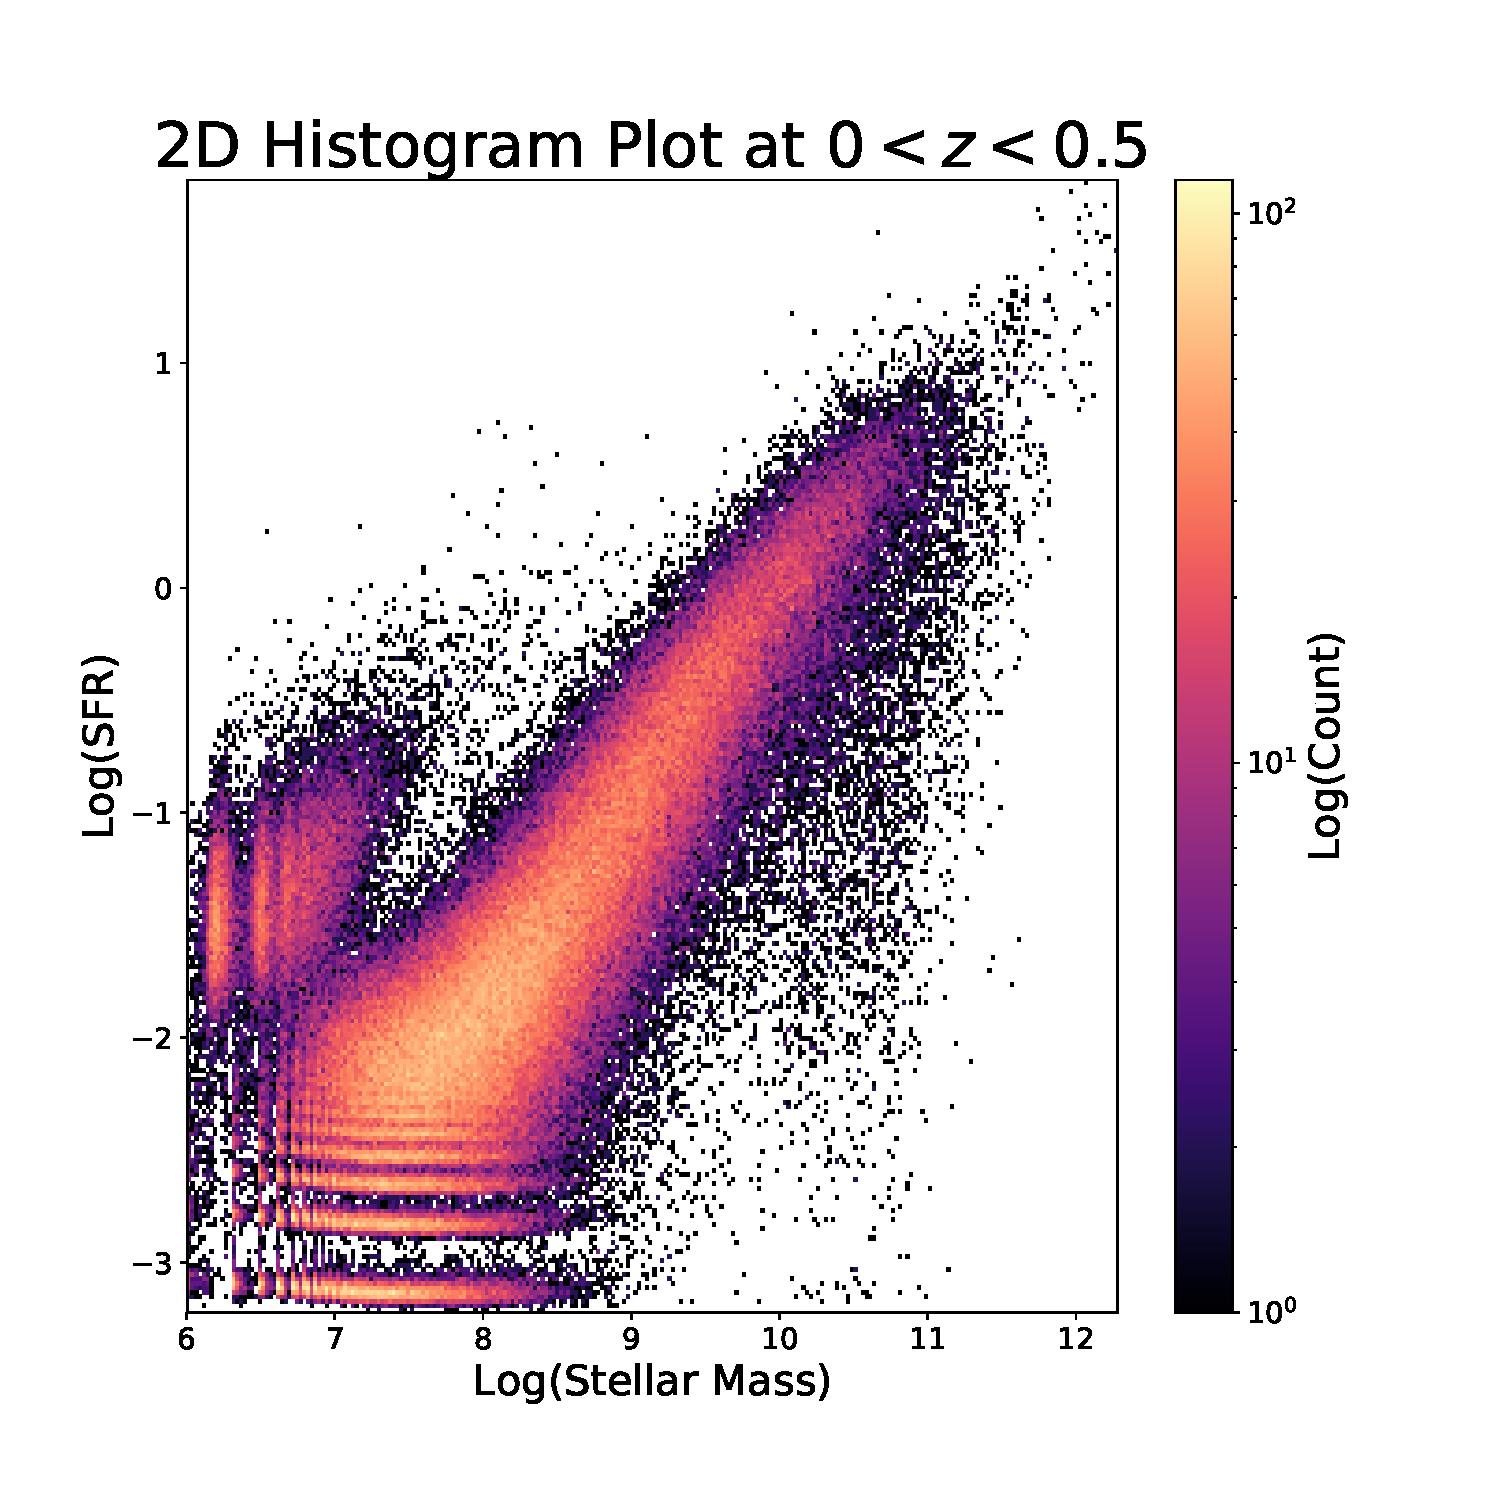
\includegraphics[width=0.5\textwidth]{histlog2.pdf}}
    \caption{Loglog histogram of the galactic Stellar Mass (SM) ($M_\odot$) against Star Formation Rate (SFR) ($M_\odot\rm{yr}^{-1}$) with a logarithmic count at $0\leq z < 0.5$.  The figure shows a higher density of galaxies along the centre of the main sequence.}
    \label{fig:histlog2}
\end{figure}

\section{Discussion and Conclusions}
{\tt SQL} queries work my retrieving columns of data from specified tables under given conditions.  In the first query used in this study, the information retrieved from the simulation was the SM and SFR, under the condition {\tt SnapNum = 28} (corresponding to $z=0$). Alternatively, this condition could have been coded as {\tt WHERE Redshift = 0}.  Importing data from one {\tt SnapNum} means that the data output will be from one snapshot in time.  

The loglog plots in Figures~\ref{fig:SMvSFR},~\ref{fig:hist}, and~\ref{fig:histlog} share a number of features that are both supported by and distinct from observational studies.  A clear relationship can be seen between the SM and SFR in the form of a thick central sequence going from the lower left of the plots up towards the upper right.  This represents the GMS.  Additionally, a cluster of galaxies can be viewed above the GMS, which agrees with observational studies of starburst galaxies.  The unusual features shown in these plots are the vertical and horizontal bands seen in the bottom left of the plots.  The reason for these bands is a result of a simplification used to make it possible to run such large volume simulations of the Universe.  The simulation makes use of subgrid models, which assume a simple model to reproduce the processes that are too small to be properly simulated, but still have long-lasting effects on the formation of galaxies. Subgrid models are described by parameters constrained directly from observations or calibration data~\cite{sim}.  The bands in these plots suggest that there must not be effective calibration data or known parameters for lower mass galaxies. 

When considering galaxies from $0 \leq z < 0.5$, there is a significant increase in galaxies being analyzed.  The first query pulled 2,275,510 galaxies (41,491 after taking the logarithm), and the second pulled 11,819,412 galaxies (269,083 after taking the logarithm).  The higher volume of galaxies made the plots much denser along the main sequence and also expanded the area of the graph covered by the main sequence.  

Selecting galaxies across a range of redshifts is more representative of what would be seen in an observational galaxy survey possibly because in reality, the galaxies would be evolving at different stages and would be at different distances and redshifts when they are observed rather than a single clean snapshot.  The maximum redshift that could be observed would be influenced by a number of factors such as if the galaxy is too far for the light to reach our telescopes (i.e., past the observable universe), if redshift causes the light to shift so far along the EM spectrum that our instruments are not capable of picking up the signal, and the amount of time the survey is left to run for.  

\clearpage
\printbibliography


\end{document}

